\chapter{Introduction}\label{chap:intro}
% add the sections
\section{Background of the Study}
\indent A workflow consists of three dimensions, namely the process, resource, and case dimension.  The process dimension is a specification of a process, the process being a partial ordering of a set of tasks such as control schemes like sequential, conditional, or iteration. The resource dimension pertains to the resource specification, where a resource is an object in the system that performs calculations, or processes, a task. Finally, the case dimension is the specification of the case, where case refers to the abstraction of a set of entities executed according to how the process is defined by the proper resource. \cite{Aalst1996} \cite{Malinao2017}.\\
\begin{figure}[]
    \centering
    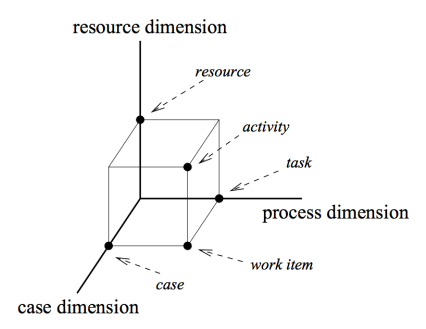
\includegraphics[width=8cm]{../figures/Workflow Dimensions.png}
    \caption{The three dimensions of workflows. (Image source:\cite{Malinao2017})}
    \label{WorkflowDimensions} 
\end{figure}
\indent Workflow models represent complex and dynamic real-world systems in various fields such as human resource management,  biology (integrated disease surveillance [Lopez et al. 2020]),  and manufacturing engineering (chiller systems \cite{Ramirez2024}). This includes models such as Petri nets (PN) and Robustness Diagrams with Loop and Time Controls (RDLT) \cite{Malinao2017}. These models allow workflow components to be analyzed and model properties to be verified. \\

\indent The study of the workflow model Robustness Diagrams with Loop and Time Controls has been important in recent years due to its capability to represent a workflow in all of its dimensions (process, resource, and case). Although there are other workflow models that can represent all dimensions e.g. business process modeling and notation (BPMN), activity diagrams, etc., there are gaps and challenges in verifying the properties of these models. Issues like concept excess, lack of support for explicit representation of data and rules, functional decomposition, etc. The dynamicity of RDLT allows it to be mapped to different mathematical models which enables different ways for the verification of model properties, such as soundness. \cite{Malinao2017} \\

\indent Classical soundness, in particular, refers to the property of a workflow to be absent of livelocks, deadlocks, and other anomalies in the flow \cite{Ramirez2024}. In general, to be classically sound, a model should have proper termination and liveliness. There are other notions of soundness derived from being classically sound, namely, relaxed, weak, easy, and lazy soundness. Relaxed soundness \cite{MalinaoPJS2023} is already defined as well as the easy, weak, and lazy notions of soundness \cite{Ramirez2024}, all of which differ in the degree of relaxations of proper termination and liveness \cite{MalinaoPJS2023}.\\  

\indent Hence, with all the knowledge about workflows and RDLT's notions of soundness, further research would expand in terms of automation to verify model properties. Therefore, various research has been done about the representation of RDLT into mathematical models aiming to automize verification. In Karen and Roben's work \cite{KarenRoben2018}, they proposed a matrix representation of RDLT to verify soundness. Asoy \cite{MalinaoPJS2023} used a matrix representation of RDLT to verify and automate classical soundness. This paper aims to leverage the structural behaviors of easy and weak soundness as formally defined by Ramirez (2024) and use matrix representations to verify these notions of soundness in an RDLT.


\section{Basic Definitions and Notations}
% -------------------------------------------
\subsection*{Robustness Diagram with Loop and Time Controls (RDLT)}
In this section, RDLT and its notions of soundness is defined. 
\indent RLDT is a workflow model that allows all three dimension of a workflow to be represented.

\begin{defn}\textbf{RDLT} \cite{Malinao2017}\\
    \label{RDLTDef}
    An RDLT is a graph representation \begin{math}R\end{math} of a system that is defined as \begin{math}R = (V, E, T, M)\end{math} where:
    \begin{itemize}
        \item \begin{math}V\end{math} is a finite set of vertices, where each vertex has a type \begin{math}V_{type}: V \rightarrow \end{math} \{'b', 'e', 'c'\} where 'b', 'e', and 'c' means the vertex is either a "boundary object", an "entity object", or a "controller", respectively.
        
        \item A finite set of arcs \begin{math}E \subseteq (V \times V) \backslash  E'\end{math} where \begin{math}E' = \{(x,y) | x,y \in V, V_{type}(x) \in \end{math} \{'b', 'e'\}, \begin{math}V_{type}(y) \in \end{math} \{'b', 'e'\}\} with the following attributes with user-defined values,
            
            \begin{itemize}
                \item \begin{math}C : E \rightarrow \Sigma \cup \{\epsilon\} \end{math} where $\Sigma$ is a finite non-empty set of symbols and $\epsilon$ is the empty string. Note that for real-world systems, a task \begin{math}v \in V\end{math}, i.e. \begin{math}V_{type}(v) = \end{math}'c', is executed by a component \begin{math}u \in V, V_{type}(u) \in \end{math} \{'b','e'\}. This component-task association is represented by the arc \begin{math}(u, v) \in E \end{math} where \begin{math}C((u,v)) = \epsilon\end{math}. Furthermore, \begin{math}C((x,y)) \in \Sigma\end{math} represents a constraint to be satisfied to reach \begin{math}y\end{math} from \begin{math}x\end{math}. This constraint can represent either an input requirement or a parameter \begin{math}C((x,y))\end{math} which needs to be satisfied to proceed from using the component/task \begin{math}x\end{math} to \begin{math}y\end{math}. \begin{math}C((x,y)) = \epsilon\end{math} represents a constraint-free process flow to reach \begin{math}y\end{math} from \begin{math}x\end{math} or a self-loop when \begin{math}x = y\end{math}.
                
                \item \begin{math}L : E \rightarrow \mathbb{Z}\end{math} is the maximum number of traversals allowed on the arc.
            \end{itemize}
        
        \item Let \begin{math}T\end{math} be a mapping such that \begin{math}T((x, y)) = (t1,...,tn)\end{math} for every \begin{math}(x, y) \in E\end{math} where \begin{math}n = L((x, y))\end{math} and \begin{math} t_{i} \in \mathbb{N}\end{math} is the time a check or traversal is done on \begin{math}(x, y)\end{math} by some algorithm’s walk on \begin{math}R\end{math}.
            
        \item \begin{math}M : V \rightarrow \{0,1\}\end{math} indicates whether \begin{math}u \in V\end{math} and every \begin{math}v \in V\end{math} where \begin{math}(u,v) \in E\end{math} and \begin{math}C((u,v)) = \epsilon\end{math} induce a sub-graph \begin{math}G_{u}\end{math} of \begin{math}R\end{math} known as a \textbf{reset-bound subsystem} (RBS). The RBS \begin{math}G_{u}\end{math} is induced with the said vertices when \begin{math}M(u) = 1\end{math}. In this case, \begin{math}u\end{math} is referred to as the \textbf{center} of the RBS \begin{math}G_{u}\end{math}. \begin{math}G_{u}\end{math}'s vertex set \begin{math}V_{G_{u}}\end{math} contains \begin{math}u\end{math} and every such \begin{math}v\end{math}, and its arc set \begin{math}E_{G_{u}}\end{math} has \begin{math}(x,y) \in E\end{math} if \begin{math}x,y \in V_{G_{u}}\end{math}.\\
        
        Finally, \begin{math}(a,b) \in E\end{math} is called an \textbf{in-bridge} of \begin{math}b\end{math} if \begin{math}a \notin V_{G_{u}}, b \in V_{G_{u}}\end{math}. Meanwhile, \begin{math}(b,a) \in E\end{math} is called an \textbf{out-bridge} of \begin{math}b\end{math} if \begin{math}b \in V_{G_{u}}\end{math} and \begin{math}a \notin V_{G_{u}}\end{math}. Arcs \begin{math}(a,b), (c,d) \in E\end{math} are \textbf{type-alike} if \begin{math}\exists y \in V\end{math} where \begin{math}(a,b), (c,d) \in Bridges(y)\end{math} with \begin{math}Bridges(y) = \{(r,s) \in E|(r,s)\end{math} is either an in-bridge or out-bridge of \begin{math}y\}\end{math} or if \begin{math}\forall y \in V, (a,b), (c,d) \notin Bridges(y)\end{math}.
    \end{itemize} 
\end{defn}

Figure \ref{sampleRDLT} shows an RLDT with a reset-bound system with center $x_2$ and its owned controllers $x_3$ and $x_4$. The in-bridges of the RBS with respect to $x_2$ are $(x_1, x_2)$ and $(x_6,x_2)$. Both arcs are type-alike with respect to $x_2$ as defined in \ref{RDLTDef}. However, $(x_3,x_2)$, being inside the RBS, is not type-alike to any of the aforementioned arcs. $(x_4, x_5)$ and $(x_4, x_6)$ are type-alike with respect to $x_4$.
For each arcs of this RDLT, $C-$ and $L-$ attributes are defined. The $x_1$ serves as the source, while the $x_7$ serves as the sink. 
\begin{figure} [H]
    \centering
    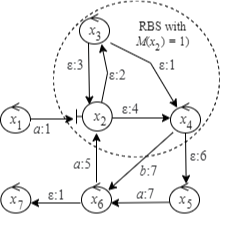
\includegraphics[width=6cm]{../figures/sampleRDLT.png}
    \caption{A Reset-Bound Subsystem-Containing Robustness Diagram with Loop and Time Controls with center at $x_2$, where $M(x_2)=1$. (Image source: \cite{MalinaoWCTP2023})}
    \label{sampleRDLT}
 \end{figure}
% Example RDLT (First Example)
% Figure \ref{RDLTComponents} shows an example of an RDLT based on the given definitions of the elements and the attributes that are labeled respectively. This RDLT also contains an RBS with the entity object $x2$ as the center of such RBS which is determined by its $M$-Attribute being equal to 1.\\
% \begin{figure}[H]
%     \centering
%     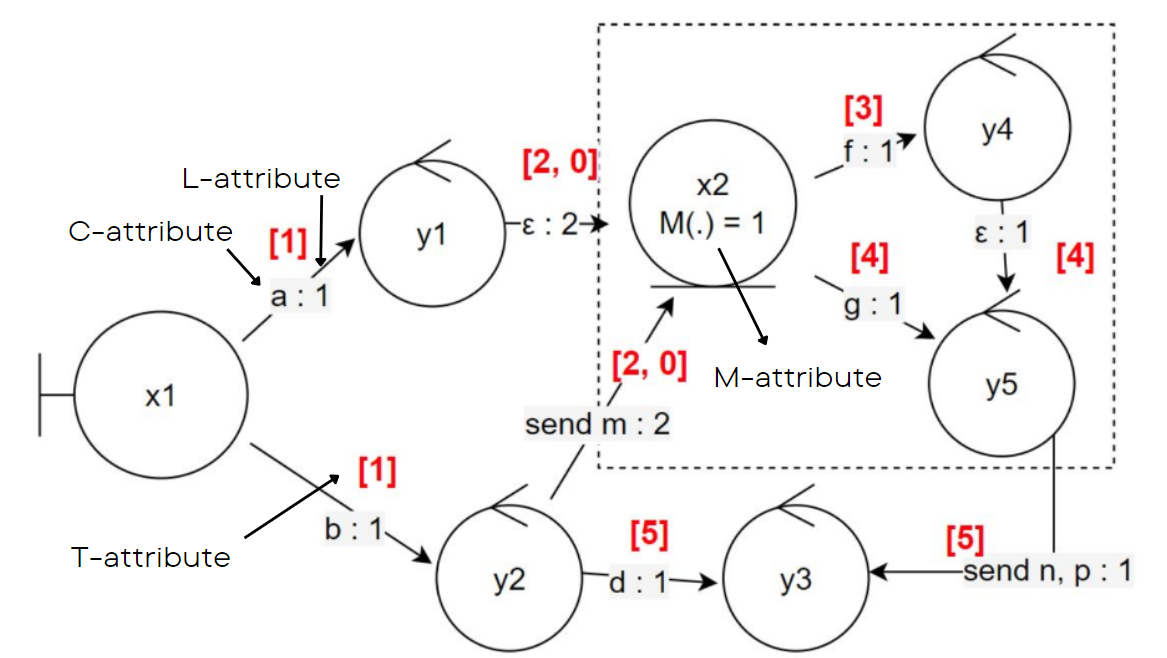
\includegraphics[width=12cm]{../figures/RDLT Components.png}
%     \caption{A Labeled Reset-Bound Subsystem-Containing Robustness Diagram with Loop and Time Controls with a Boundary Object $x1$, an Entity Object $x2$, and Controllers $y1$, $y2$, $y3$, $y4$, and $y5$. (Image source: \cite{Sulla2023})}
%     \label{RDLTComponents}
% \end{figure}

% -------------------------------------------
\subsection*{Activity Extraction Algorithm}
The proposed Activity Extraction algorithm in \cite{Malinao2017} takes an input RDLT \emph{R} with a defined start index \emph{s} and goal vertex \emph{f}. As shown in Algorithm \ref{ActivityExtraction} it returns an activity profile defined in \ref{activityProfile}, a set of exected vertices from the extracted activities.
To understand activity extraction fully, along with the definition of activity profile, reachability configuration, defined in \ref{reachabilityConfiguration}, is also first introduced.
\begin{defn}\label{reachabilityConfiguration}
    \textit{\textbf{Reachability Configuration}}\\
    A reachability configuration $S(t)$ in $R = (V, E, \Sigma, C, L, M)$ contains the arcs traversed by ${\mathcal A}$ at time step $t \in {\mathbb{N}}$.
\end{defn}
\begin{defn}\label{activityProfile}
    \textit{\textbf{Activity Profile}}\\
    A set $S = \{S(1), S(2), \ldots,$ $S(d)\}$ of reachability configurations, $d \in {\mathbb{N}}$, is an activity profile in $R = (V, E, \Sigma, C, L, M)$ where $\exists(u,v) \in S(1)$ and $(x,y) \in S(d)$ such that $\nexists w, z \in V$ where $(w,u), (y, z) \in E$. 
\end{defn}
Another definition, that of \emph{Unconstrained Arc} in \ref{unconstrainedarc} defines what an unconstrained arc is which allows for the traversal of arcs in activity extraction.

\begin{algorithm}[H]
    \caption{Activity Extraction Algorithm ${\mathcal A}$ \cite{Malinao2017, Sulla2023}}
    \label{ActivityExtraction}
    \begin{algorithmic}
        \State \textbf{Input:} $ R $, $ s \in V $, $ f \in V $
        \State \textbf{Output:} vertices $ S $ of $ R $, $ \emptyset $ otherwise
    \end{algorithmic}
    \begin{algorithmic}[1]
        \State Initialize $ S $
        \For{every $ (x,y) $}
            \State Initialize $ T((x,y)) $ such that $ T((x,y)) $ $ = $ $ (t_1, ..., t_n) $ where $ n $ $ = $ $ L((x,y)) $ and $ t_i $ $ \epsilon $ $ \mathbb{N} $ is the time a check or traversal is done on $ (x,y) $ by $ A $.
        \EndFor
        \State Let $ x $ $ = $ $ s $.
        \While{$ x $ $ \neq $ $ f $}
            \State Select $ (x,y) $ $ \epsilon $ $ E $ where $ L((x,y)) $ has not been reached.
            \If{$ \exists (u,x) $ $ \epsilon $ $ E $ $ = $ $ max(T((u,x))) $}
                \State Assign $ maxV $ $ + $ $ 1 $ to the leftmost zero of $ T((x,y)) $. 
            \Else
                \State $ maxV $ $ = $ $ 0 $.
            \EndIf
            \State Determine whether $ (x,y) $ is an unconstrained arc or not.
            \If{$ (x,y) $ is unconstrained}
                \State Traverse $ (x,y) $ .
                \State Assign $ MAX $ $ + $ $ 1 $ to $ T((x,y)) $ where $ MAX $ is the maximum value from all $ T((v',y)) $ $ \forall $ $ v' $ $ \epsilon $ $ V $ where $ (v',y),(v,y) $, and $ (x,y) $ are type-alike.
                \For{every $ (v,y) $ $ \epsilon $ $ E $ that is type-alike with $ (x,y) $}
                    \State Assign $ MAX $ $ + $ $ 1 $ to every $ T((x,y)) $.
                    \If{$ C((v,y)) $ $ \epsilon $ $ \Sigma $}
                        \State The last value in $ T((x,y)) $ where the last check was done on $ (v,y) $ is updated.
                    \ElsIf{$ v $ is either type 'b' or 'e' and $ y $ is type 'c'}
                        \State The first value in $ T((x,y)) $ is updated.
                    \EndIf
                \EndFor
            \ElsIf{$ (x,y) $ is not unconstrained and not other $ (x,y') $ $ \epsilon $ $ E $ where $ y' $ $ \epsilon $ $ V $ can be selected }
                \State Backtrack to $ a $ $ \epsilon $ $ V $ where $ (a,x) $ $ \epsilon $ $ E $ and $ a $ was previously visited by the algorithm to reach $ x $.
            \EndIf
        \EndWhile
        \If{activity extraction fails}
            \State \Return $ \emptyset; $
        \Else
            \State \Return $ S $
        \EndIf
    \end{algorithmic}
\end{algorithm}
\newpage
In step 4.3 of algorithm ${\mathcal{A}}$, an evaluation is performed to determine if $(x,y) \epsilon E$ is an unconstrained arc. The definition of an unconstrained arc is defined as follows:
\begin{defn} \label{unconstrainedarc}
    \textit{\textbf{Unconstrained Arc}}\\
    An arc $(x, y) \in E$ is \textbf{unconstrained} if $\forall (v,y) \in E$, where $(x,y)$ and $(v,y)$ are type-alike, any of the following traversal conditions hold, 
    \begin{enumerate}
        \item $C((v,y)) \in \{\epsilon, C((x,y))\}$,
        \item { $|\{t_i \in T((x,y))|t_i \geq 1\}| \leq  |\{t_j \in T((v,y))|t_j \geq 1\}|$ $\leq L((v,y)),$}
        \item $C((v,y)) \in \Sigma, C((x,y)) = \epsilon \wedge T(v,y) \neq [0]$.
    \end{enumerate}
    Note that $(x,y)$ will remain unconstrained (if it is such) regardless of any other $(v,y)$ where $(x,y)$ and $(v,y)$ are not type-alike.
\end{defn}
% -------------------------------------------
\subsection*{Vertex Simplification}
\begin{defn}\textbf{Vertex Simplified $R$} \cite{Malinao2017}\\
    \label{VertexSimpDef}
     A vertex-simplified RDLT $ G $ = ($ V' $, $ E' $, $ C' $) of $ R = (V, E, T, M) $ (with arc attributes $ C $ and $ L $) is a multigraph whose vertices $ v \in $ V have $ V_{type}(v) = 'c' $ where $ G $ is derived from $ R $ such that the following holds:
     \begin{enumerate}
         \item $ x \in V' $ if any of the following holds:
         \begin{itemize}
             \item $ x \in V $ and $ x \notin V_{G_u} $ of an RBS $ G_u $ in $ R $, or
             \item there exists an in-bridge $ (q, x) \in E $ of $ x \in V \cap V_{G_u}, q \in V $ of $ R $, or
             \item there exists an out-bridge $ (x, q) \in E $ of $ x \in V \cap V_{G_u}, q \in V $ of $ R $, or
         \end{itemize}
         \item $ (x, y) \in E' $ with $ C'((x, y)) = C((x, y)) $ for $ x, y \in V' $ if $ (x, y) \in E $
         \item $ C((x, y)) = \varepsilon $ if $ x, y \in V' \cap V_{G_u} $ and $ x $ is an ancestor of $ y $ in $ R $ and $ (x, y) \notin E_{G_u} $  
     \end{enumerate}

     We refer to this simplification of $ R $ as \textbf{level-1 vertex simplification} of $ R $ with respect to every RBS $ G_u $ in $ R $. A \textbf{level-2 vertex simplification} of $ R $ with respect to its RBS $ G_u $ is the level-1 vertex-simplification of $ G_u $ where $ G_u $ is treated as an RDLT where the value of the vertex attribute $ M $ of $ u $ is redefined to $ 0 $, i.e. $ M(u) $ $ = $ $ 0 $. With this, the verification of model properties (i.e. maximally composed and sound RDLTs) are separately done for the level-1 and level-2 vertex simplifications of $ R $. However, this separation does not affect the validity of proving for any of these properties on the entire RDLT itself. Furthermore, 
 \end{defn}

 In simpler terms, the vertices in \emph{R} present in a vertex-simplified RDLT \emph{G} are those that do not belong in any RBS or those inside an RBS but has an \emph{in-bridge} and/or an \emph{out-bridge}.
 The vertex-simplifications $R_1$ and $R_2$ of the RDLT in \ref{sampleRDLT} is shown in \ref{vertexSimplification}, respectively. $R_1$ captures a subgraph of $R$ found outside of its RBS, including the vertices of the RBS that have at least 1 in-brigde or out-bridge. $R_2$ vertex-simplification, however, captures the RBS itself. The vertices that have in- or out-bridges in $R$ are marked either as sources and/or sinks in $R_2$.
 \begin{figure}[H]
    \centering
    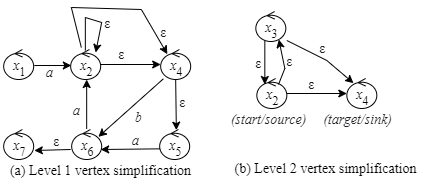
\includegraphics[]{../figures/vertexSimplification.png}
    \caption{The levels 1 and 2 vertex simplification $R_1$ and $R_2$ of the RLDT in \ref{sampleRDLT} (Image Source: \cite{MalinaoWCTP2023})}
    \label{vertexSimplification}
\end{figure}
% -------------------------------------------
\subsection*{L-Safeness of RDLTs}
% include here the defintions from kuya Ronnie's
% add paragraph introducing L-safeness of RDLT
In the analysis of processes in RDLT, particularly on its verification of soundness property, it is crucial that possible $L$-attrbute-based deadlocks are avoided. Reachability of the vertices relies heavily on the configuration of the arcs' $L-$values. The following definitions discusses the $L-$safeness with RDLTs from \cite{MalinaoPJS2023}.
\begin{defn}\textbf{Critical and Escape Arcs} \cite{MalinaoPJS2023}
    A cycle $ c $ $ = $ $ [ x_1 x_2 \ldots x_n ] $ is a sequence of vertices $ x_i $ $ \in $ $ V $, where $ (x_i,x_{i+1}) $ $ \in $ $ E $, $ i $ $ = $ $ 1,2, \ldots, n - 1 $, and no two vertices in $ c $ are the same except for $ x_1 $ $ = $ $ x_n $. The elements of $ c $ are denoted as $ Lit(c) $. We denote the set of arcs of $ c $ as $ ArcsOfCycle(c) $ $ = $ $ \{ (x,y) $ $ \in $ $ E | \exists x_i, x_{i+1} $ $ \in $ $ Lit(c) $ where $ x $ $ =  $ $ x_i $ and $ y $ $ = $ $ x_{i+1} \} $.

    $ (x,y) $ $ \in $ $ ArcsOfCycle(c) $ is called a critical arc (CA) in $ c $ if it has the minimum $ L $-value among the arcs in $ c $, i.e. $ L(x,y) $ $ = $ $ min_{(u,v) \in ArcsOfCycle(c) } \{L(u,v)\} $. If $ \exists (x,v) $ $ \in $ $ E $ such that $ v $ $ \in $ $ V \backslash Lit(c) $, then we refer to $ (x,v) $ as an escape arc (EA) of $ (x,y) $ in $ c $. Self-loops, i.e. $ (x,x) $, are cycles that are themselves entirely composed of one critical arc that does not affect the (re)use of other arcs in an RDLT.
\end{defn}

\begin{defn}\textbf{Loop-Safe Arcs} \cite{MalinaoPJS2023}
    \label{LSA}
    Let $ R $ be a connected RDLT, i.e. for every vertex $ v $ $ \in $ $ V $, there is a path from a source vertex $ s $ $ \in $ $ V $ to $ v $ in $ R $. A non-critical arc (NCA) $ (x,y) $ $ \in $ $ E $ of $ R $ is loop-safe if $ L(x,y) $ $ > $ $ RU(x,y) $, where
    \begin{gather*}
        RU(x,y) = \Sigma_{k=1^{|Cycles(x,y)|}} (I * L(u,v)) \text{, for some } (u,v) \in minL\_CA(c_k) \text{, with} \\
        I =
        \begin{cases}
            1, & \text{if } k = 1 \text{ or } \cup_{j=1^{k-1}} minL\_CA(c_j) \cap minL\_CA(c_k) \\
            0, & \text{otherwise,}
        \end{cases}
    \end{gather*}
    and $ minL\_CA(c) $ $ \subset $ $ E $ is the set of arcs whose $ L $-value is the minimum among the critical arcs found in $ c $, accounting the other cycles in $ c' $ in $ R $ that intersect with $ c $.
\end{defn}

\begin{defn}\textbf{Safe Critical Arcs} \cite{MalinaoPJS2023}
    \label{SafeCA}
    A CA $ (x,y) $ $\ in $ $ E $ is safe if there is an escape, non-critical arc $ (x,z) $ $\ in $ $ E $, where $ (x,z) $ is loop-safe.
\end{defn}
\subsubsection*{JOINs in RDLTs}
In RDLTs, it is not impossible for multiple processes to converge at a single vertex (JOIN). The type of join specifies how the incoming processes interact before proceeding in the workflow. The following definitions are the different types of joins in RDLTs:
\begin{itemize}
    \item[1.] AND-JOIN at $y \in V$: For every type-alike arcs $(v,y), (u,y) \in E$ where $(v,y) \neq (u,y)$, their C-values $C(v,y) \neq C(u,y)$ and $C(v,y),C(u,y) \in \Sigma$.
    \item[2.] MIX-JOIN at $y \in V$: There is at least one pair of type-alike arcs $(v,y), (u,y) \in E$ where $(v,y) \neq (u,y)$, $C(v,y) \neq C(u,y)$ and $C(v,y) = \epsilon$, and $C(u,y) \in \Sigma$.
    \item[3.] OR-JOIN: For every type-alike arcs $(v,y), (u,y) \in E$ where $C(v,y)=C(u,y)$.
\end{itemize}
The concept of JOIN-safe L-values ensures processes are in proper coordination with each other. This, along with \ref{LSA} and \ref{SafeCA}, provides the structural requirement for a classically sound RDLT, e.g, proper termination and liveness. These definitions serves as the basis for determining looser notions of soundness.
\begin{defn}\textbf{JOIN-safe L-values} \cite{MalinaoPJS2023}
    \label{JSL}
    For every pair of arcs $(u, y)$, $(v, y)$ $ \in $ $ E $, where $C(u, y)$ $ \neq $ $C(v, y)$, we say that $(u, y)$ and $(v, y)$ have JOIN-safe $L$-values if:

    \begin{enumerate}
        \item \textbf{One split origin.} There is exactly one common ancestor $ x $ $ \in $ $ V $ for $ u $ and $ v $ such that there is exactly one path $ P_u $ $ = $ $ a_1 a_2 \ldots a_n $, where $ a_1 $ $ = $ $ x $, $ a_{n-1} $ $ = $ $ u $, $ a_n $ $ = $ $ y $, $ a_i $ $ \in $ $ V $, $ 1 < I < n - 2 $, and another path $ P_v $ $ = $ $ b_1 b_2 \ldots b_m $, where $ b_1 $ $ = $ $ x $, $ b_{m-1} $ $ = $ $ v $, $ b_m $ $ = $ $ y $, $ b_j $ $ \in $ $ V $, $ 1 < j < m - 2 $. Furthermore, $ P_u $ and $ P_v $ do not intersect with each other except at $ x $ and $ y $. That is, no $ a_i $ and $ b_j $ along these paths are equal, for $ 1 < i < n $ $ 1 < j < m $; and
        \item \textbf{No unrelated process.} For every arc $ (a,b) $ $ \in $ $ E $, if $ a $ $ = $ $ x $, where $x$ is the one common ancestor of $u$ and $v$, then there is no path from $a$ to another vertex $r$ $\in$ $V$ such that for some $(r,s)$ $\in$ $ E $, $s$ $\neq$ $y$.
        \item \textbf{No branching out from every related process.} $\forall q_k $ $ \in $ $ Lit(P_q) $, where $ q $ $ \in $ $ \{u,v\} $, $ 1 \leq k < |Lit(P_q)| $, $ \nexists (q_{k,s}) $ $ \in $ $ E $ where $ s $ $ \in $ $ V \backslash Lit(P_q) $.
        \item \textbf{No process interruptions.} $ \forall q_k $ $ \in $ $ Lit(P_q) $, where $ q $ $ \in $ $ \{u,v\} $, $ 1 < k \leq |Lit(P_q)| $, $ \nexists (s,q_{k}) $ $ \in $ $ E $ where $ s $ $ \in $ $ V \backslash Lit(P_q) $.
        \item \textbf{Duplicate conditions.}
        \begin{itemize}
            \item If $ C(u,y) $, $ C(v,y) $ $ \in $ $ \Sigma $, i.e. an AND-JOIN at $ y $, then there is no process $ P $ $ = $ $ [x_1 x_2 \ldots x_p] $ in $ R $, where $ x_1 $ $ = $ $ x $, $ x_p $ $ = $ $ y $, such that $ C(x_{p-1}, x_p ) $ $ = $ $ C(u,y) $ (or $ C(v,y) $).
            \item Without any loss of generality, if $ C(u,y) $ $ = $ $ \varepsilon $ and $ C(v,y) $ $ \in $ $ \Sigma $, then any process $ P $ $ = $ $ x_1 x_2 \ldots x_p $ in $ R $, where $ x_1 $ $ = $ $ x $, $ x_p $ $ = $ $ y $, can have $ C(x_{p-1}, x_p) $ $ \in $ $ \{\varepsilon, C(v,y)\}$. That is, a MIX-JOIN can have duplicate conditions for the arcs connecting to $y$, but no two of such arcs have different conditions.
        \end{itemize}
        \item \textbf{Equal $ L $-values of arcs at the AND-JOIN.}
        \item \textbf{Loop-safe components of every related process.} For an AND- or MIX-JOIN merging at $y$, each of its processes $ P $ $ = $ $ x_1 x_2 \ldots x_k $, $ k $ $ \in $ $ \mathbb{N} $, where $ x_1 $ $ = $ $ x $ and $ x_k $ $ = $ $ y $, the arc $ (x_1, x_{i+1}) $ $ \in $ $ E $. $ i $ $ = $ $ 1, 2, \ldots, k - 1 $, is loop-safe. Lastly, for an OR-JOIN merging at $ y $, each process $ P $ $ = $ $ x_1 x_2 \ldots x_k $, $ k $ $ \in $ $ \mathbb{N} $, of this JOIN has its arc $ (x_i,x_{i+1}) $ to have a JOIN-safe L-value, $ i $ $ = $ $ 1, 2, \ldots, k - 1 $, if $ (x_i, x_{i+1}) $ is either a loop-safe arc or a safe CA in R.
    \end{enumerate}
    
\end{defn}
% -------------------------------------------
\subsection*{Reusability and Resets in RDLTs}
The concept of reusability refers to how components of an RDLT can be used in different situations, such as when an RDLT has an RBS \cite{MalinaoWCTP2023}. The information in this section is sourced from \cite{MalinaoWCTP2023} unless explicitly mentioned otherwise.

\begin{defn} Pseudocritical Arcs, Pseudo-escape Arcs \\
A pseudocritical arc $(PCA) (x,y) \in E$, where $(x,y)$ is a component of a cycle $c$ in $R$ where $L(x,y$) is the minimum among all the L-values of the arcs in $c$ which are not arcs of an RBS in $R$.

Meanwhile, a pseudo-escape arc $(PEA) (x,z) \in E$ is a non-critical arc in $R$ where $(x,y)$ and $(x,z)$ are type-alike.    
\end{defn}

\begin{defn} Expanded Reusability in RDLTs with Resets \\
Let $R =  (V, E, T, M)$ be a connected $RDLT$. If $\exists v \in V$ where $M(v)=1$, then let $B =  (V', E', T', M')$ be the RBS with its center $v$.
\begin{enumerate}
    \item Let $IB_r(X)$ be the set of in-bridges of $x \in V$.
    \item Let $Cycles_{part}(R)$ be a set of cycles in $R$ with the following property: $\forall p = [x_1 x_2 ... x_n] \in Cycles_{part}(R)$, there exist cycle components meeting these conditions:
    \begin{itemize}
        \item [(a)] $(x_i,x_{i+1}) \in E$ is inside an RBS $B$ of $R$ (i.e, $x_i,x_{i+1} \in V'$).
        \item [(b)] $(x_j,x_{j+1}) \in E$ is not inside $B$ (i.e, $x_j or x_{j+1} is not in V'$).
    \end{itemize}
\end{enumerate}
Whenever we have cycles $d = [d_1 d_2 ... d_{m1}], e = [e_1 e_2 ... e_{m1}] \in Cycles_{part}(R)$ that overlap in their non-RBS components, and this overlap contains both of their PCAs $(d_k,d_{k+1}), (e_{k'},e_{k'+1})$, where $L(d_k,d_{k+1}) \geq L(e_{k'},e_{k'+1})$, then consider only one of these PCAs. Choose the one with the minimum L-value as it would ultimately contribute to the reusability of every RBS component reachable from these cycle components.
\end{defn}

\begin{defn} (RU-preserving transformation) \\
    A transformation $\delta$ of an input RDLT $R$ to another RDLT $R'$ is said to be RU-preserving if for every activity profile $S = {S(1), S(2), ..., S(n_1)}, n_1 \in IN$, that is derivable from $R$, there is a corresponding activity profile $S' = {S'(1), S'(2), ..., S'(n_2)}, n_2 \in IN$, that is derivable from $R'$, where for every pair $(x,y) \in S(i)$ and $(y,z) \in S(i+1)$, either of the following holds:
    \begin{enumerate}
        \item $(x,y) \in S'(j)$ and $(y,z) \in S'(j+1)$,
        \item there exists a path $p=x_1, x_2, ..., x_n \in R$ being represented by the arc $(x_1, x_n)$ in $R$ being represented by the arc $(x_1, x_n)$ in $R'$ where $x_{k-1}=x,x_k, x_{k+1}=z$, and
            \begin{itemize}
                \item[(a)] $(s,x_1) \in S'(j)$ and $(x_1,x_n) \in S'(j+1)$, for some vertex $s$ in $R'$,
                \item[(b)] $(x_1,x_n) \in S'(j)$, for some $1 \leq j \leq n_2$, or
                \item[(c)] $(x_1,x_n) \in S'(j)$ and $x_n$, $s \in S_{j-1}$, for some vertex $s$ in $R'$.
            \end{itemize}
    \end{enumerate}
    Furthermore, we call $(x_1,x_n)$ as the abstract arc in $R'$ representing the path $p$ in $R$.
\end{defn}
% -------------------------------------------
\subsection*{Expanded Vertex Simplification}
The process of vertex simplification results to an RDLT lacking of $L$-values, both in $R_1$ and $R_2$. Therefore, \cite{MalinaoWCTP2023} proposes and extension of the process to produce \emph{expanded vertex simplifiction} $R_1'$ and $R_2'$ of $R$ by using the RDLT and its simplified vertex to retrieve the other attributes, e.g. $L$. The algorithm for producing $R_1'$ and $R_2'$ is outlined in \ref{EVSA}.
\begin{algorithm}
    \label{EVSA}
    \underline{\textbf{Expanded Vertex Simplification Algorithm(EVSA):}}\\
    \textbf{Inputs:} Let $R = (V, E, T, M)$ be an connected RDLT with an RBS, i.e. $\exists v \in V$, where $M(v) = 1$. Let $R_1 = (V_1, E_1)$ and $R_2 = (V_2, E_2)$ be the vertex simplifications of $R$. (The $C$-attributes of the arcs of $R$, $R_1$, and $R_2$ are denoted as $C$, $C_1$, $C_2$, respectively, while their $L$-attributes are $L$, $L_1$, and $L_2$, respectively.) \\

    \noindent
    \textbf{Outputs:} \textbf{Level 1 and Level 2 expanded vertex simplification} $R'_1 = (V'_1, E'_1, T'_1)$ and $R'_2 = (V'_2, E'_2, T'_2)$ of $R$, respectively . (The $C$-attributes of the arcs of $R'_1$ and $R'_2$ are $C'_1$ and $C'_2$, respectively, while their $L$-attributes are $L'_1$ and $L'_2$, respectively.)

    \begin{enumerate}
        \item For each $v \in V_1(V_2)$(or $V$ of $R$), set $v' \in V'_1(V'_2)$ to be its corresponding vertex, and if $(u,v) \in E_1(E_2)$, then its there is a corresponding arc $(u',v') \in E'_1(E'_2)$, where the $C$-values $C'_1(u',v')(C_2(u',v'))$ of $R'_1(R'_2)$ is set to $C(u,v)$ of $R_1(R_2)$, otherwise, none.  \\

        This step copies the vertices and arcs, inclusive of the $C$-values of $R_1$ and $R_2$ to their corresponding expanded versions $R'_1$ and $R'_2$, respectively. 

        \item For each $(u,v) \in E$, where $(u,v)$ is not in an RBS of $R$, and its corresponding arc $(u',v') \in V'_1$ of $L_1$, let $L'_1(u',v') = L(u,v)$. \\

        This step copies the $L$-values of $R$ for each of its arcs to the $L$-values of $R'_1$ whenever such arc does not belong to an RBS of $R$. 
        
        \item For each abstract arc $(u',v') \in E'_1$ of $R_1$, where $(u',v')$ represents the path \mbox{$p = x_1 x_2 \ldots x_n$} in $R$, i.e. $x_1 \in V$ and $x_n \in V$ correspond to $u' \in E'_1$ and  $v' \in E'_1$, respectively, set $L'_1(u',v') = \min\limits_{i = 1, \ldots, n-1} \{eRU(x_i, x_{i+1})\} + 1$. \\
        
        This step sets the $L$-value  of each abstract arc $(u',v')$ of $R'_1$ to reflect the maximum number of reuse of the path that it represents in $R$. Note that we treat each component of the RBS as an NCA relative to the non-RBS components, $eRU(u',v')$ must be greater than its reusability, e.g. greater than the PCAs of the cycles $(u',v')$ are involved in, hence, we add 1 to this maximum number of reuse. Additionally, note the $eRU$ of the arcs along the path $p$ can vary because of the reuse of such components within the RBS, albeit the number of times they are accessible through the in-bridges of their ancestor node is the same. However, the reusability of the entire path $p$ itself is bound to the minimum of the $L$-values of the arcs therein. Thus, this minimum shall be the representative $L$-value for these arcs as reflected by their representative abstract arc.
    \end{enumerate}
\end{algorithm}

\begin{figure}[H]
    \centering
    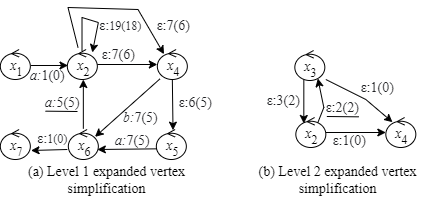
\includegraphics{../figures/expandedVertexSimplification.png}
    \caption{$R_1'$ and $R_2'$ expanded vertex simplification of the vertex simplified graphs in figure \ref{vertexSimplification}}
    \label{expandedVertexSimplifiedRLDTs}
\end{figure}
In simpler terms, the creation of a contraction path of a given vertex simplified RDLT $ G_1 $ or $ G_2 $, which can also be represented as $R_1$ and $R_2$ respectively, is the merging of a pair of vertices $ x $ and $ y $ connected by the arc $ (x,y) $ from the initial vertex through the contraction of arcs. Such a merging is only possible if the set of C-values of all arcs from $ x $ to $ y $ is a superset of the C-values of all arcs from other vertices in the subgraph towards $ y $ \cite{MalinaoWCTP2023}. This continues until the subgraphs $ R_1 $ and $ R_2 $ are represented as one vertex, if possible. This method is also referred to as the graph contraction strategy.

% -------------------------------------------
\subsection*{Soundness Property in RDLT}
On the soundness of RDLT, there are two formalized definitions of soundness, namely Classical and Relaxed Soundness \cite{Malinao2017,MalinaoPJS2023}. However, a recent formalization was also made for weak and easy soundness \cite{Ramirez2024}, the definitions of which are stated below.
\begin{defn}\textbf{Classical Soundness of RDLTs} \cite{MalinaoPJS2023}
    \label{ClassicalRDLTDef}
    An RDLT is of classical sound if and only if the following requirement is satisfied by each activity profile $ S = \{S(1), S(2), ..., S(k)\}, 1 \leq k \leq diam(R), diam(R) $ is the diameter of $ R $, of a set of source vertices $ I $ $ \subset $ $ V $ and a final output vertex $ f $ $ \in $ $ V, $ where $ \forall $ $ x $ $ \in $ $ I $ and $ y $ $ \in $ $ V $, $ (x,y) $ $ \in $ $ S(1), $ and $ (u,f) $ $ \in $ $ S(k) $, $ u $ $ \in $ $ V $:
    \begin{enumerate}
        \item \textbf{Proper termination.} For every activity profile $ S = \{S(1), S(2), ..., S(k)\}, 1 \leq k \leq diam(R) $, of a set of source vertices $ I $ $ \subset $ $ V $ and a final output vertex $ f $ $ \in $ $ V $.
        \begin{itemize}
            \item All arcs in the final reachability configuration $ S(k) $ must be incident to sink $ f $, i.e. for every $ (x,y) $ $ \in $ $ S(k), $ $ y = f $
            \item If $ k $ $ \leq $ $ 2 $: every arc incident to a vertex $ y $ in a reachability configuration $ S[i] $ has a corresponding arc incident from vertex $ y $ in a succeeding reachability configuration $ S(j) $, $ i.e. $ for every $ (x,y) $ $ \in $ $ S[i] $, there exists another arc $ (y,z) $ $ \in $ $ S(j) $, for all $ 1 \leq i < k $, and for some $ j $ in the range $ i + 1 \leq j \leq k $.
        \end{itemize}
        \item \textbf{Liveness.} Every arc is traversed in some activity profile, $ i.e. $ for every $ (x,y) $ $ \in $ $ E $, there is an activity profile $ S' = \{S'(1), S'(2), ..., S'(k')\} $, where $ (x,y) $ $ \in $ $ S'[i], 1 \leq k \leq k' $.
    \end{enumerate}
\end{defn}

Based on this definition, the first condition requires an RDLT \emph{R}'s each specified vertex and their subsequent vertices leading to the final vertex of \emph{R}. In other words, an RDLT needs to have proper termination. 
The second condition requires it to have no possible occurences of deadlocks for every component in the RDLT as it requires that all arcs are to be traversed to be included in the activity profile during extraction. Figure \ref{sampleRDLT} satisfies both conditions an is therefore classically sound.

\begin{defn}\textbf{Relaxed Soundness of RDLTs} \cite{Malinao2017, MalinaoPJS2023, Sulla2023}
    \label{RelaxedRDLTDef}
    An RDLT is of relaxed sound if for every sink $ f $ $ \in $ $ V $ and a source $ w $ $ \in $ $ R $, where $ w $ is an ancestor of $ f $, there exists an activity profile $ S = {S(1), S(2), ..., S(k)} $, where $ 1 \leq k \leq diam(R) $, where the following conditions hold:
    \begin{itemize}
        \item For every reachability configuration $ S(t) $ prior to $ S(k) $, if any, there should be at least one arc $ (x,y) $ $ \in $ $ S(t) $ and another arc $ (y,z) $ $ \in $ $ S(t') $, for a time $ t' $, where $ t < t' \leq k $. This ensures that there is at least one continuous path from $ w $ to $ f $ in activity $ S $.
        \item The final reachability configuration $ S(k) $ is only composed of arcs that point to the sink $ f $, $ i.e. $ $ \forall (x,y) $ $ \in $ $ S(k) $, $ y = f $.
        \item The set of arcs traversed at a time $ t $ is strictly contained in the set of arcs traversed at time $ t + 1 $, $ i.e. $ $ \bigcup_{i=1}^{t} S[i] $ $ \subset $ $ \bigcup_{i=1}^{t+1} S[i] $. Since an arc can occur in multiple $ S[i] $, the operator $ \bigcup $ should be considered a multiset union operator.
        \item Every arc $ (x,y) $ $ \in $ $ E $ is traversed in some activity profile $ S' $, $ i.e. $ there exists an activity profile $ S' $, where $ (x,y) $ $ \in $ $ S'(t) $ for some $ S'(t) $ $ \in $ $ S' $.
    \end{itemize}
\end{defn}
Relaxed soundness refers to a classically sound RDLT with the exception of the loosening of its proper termination. At least only one vertex is required to be leading to the final vertex, in contrast to a classically sound RDLT. This is given by the first, third, and fourth requirement. The liveness, however, is retained as defined in the second and third requirement, preventing deadlocks. Meaning, a relaxed soundness is live.  The RDLT therefore in figure \ref{sampleRDLT} is relaxed sound, aside from the fact that it is classically sound in the first place.

% -------------------------------------------


\section{Problem Statement}
Matrix representation is used to extract activities from an RDLT, using computations involving matrix operations. The purpose of this research is to verify the weak and easy soundness of an input RDLT using these operations. Karen and Roben \cite{KarenRoben2018} and Asoy \cite{Asoy2024} already conducted studies involving the matrix representation of relaxed and classical soundness, respectively. Similarly, the recently formalized notion of soundness, that of weak and easy soundness in RDLT \cite{Ramirez2024}, provided a behavioral and structural profile upon which algorithms were proposed for the verification thereof. The problem statement of this paper is to create a matrix representation for the verification of weak and easy soundness of RDLT, based on its formalizations.
% objectives of the study
\section{Aim of the Work}
\subsection*{General Objectives}
Currently, there are already existing literature on weak and easy soundness in the context of RDLT. However, in the case of this research, the matrix representation for the verification of these notions of soundness is to be addressed. Therefore, we shall address the following general objectives:
\begin{enumerate}
    \item To incorporate matrix operations on the matrix representation of RDLT to verify easy and weak soundness;
    \item To design a matrix representation of RDLT to verify easy and weak sound- ness; and
    \item To create an algorithm for the verification of RDLT using matrix repre- sentation.
\end{enumerate}
\subsection*{Specific Objectives}
In alignment with the general objectives, the following specific objectives are identified to reach these aims:
\subsubsection*{For Weak Soundness Structural Verification}
\begin{enumerate}
    \item To establish matrix representation and operations for the verification of deadlock tolerance in both level 1 and level 2 expanded vertex simplification graphs, $R_1$ and $R_2$, respectively, of RDLT $R$.
    \item To establish matrix representation and operations for the verification that $R$ is deadlock-resolving.
    \item To generate a list of deadlock points in $R$ and identify escape contraction paths.
    \item To establish matrix representation and operations for the verification of weakened-join safeness of $R$.
    \item To establish matrix representation and operations to verify weakened join-safe values of every split-join pair in $R$.
    \item To verify the loop-safeness of NCA and safeness of CA\@.
    \item To measure the time and space complexity of the matrix-based verification of weak soundness of $R$.
\end{enumerate}
\subsubsection*{For Easy Soundness Structural Verification}
\begin{enumerate}
    \item To establish matrix representation and operations for the verification of a contraction path existing from the source to the sink vertex.
    \item To measure the time and space complexity of the matrix-based verification of easy soundness of R.
\end{enumerate}
% scopes and limitations
\section{Scope and Limitations}
The scope and limitations of the study are the following:
\begin{enumerate}
    \item The study will focus on the design of matrix representation that encapsulates the structure of RDLT. It will incorporate matrix operations on the verification of the structural profiles of RDLT to determine its weak and easy soundness. The study will not delve to alternative models other than matrix representation.
    \item The study will center on RDLT as the main structural model to verify notions of soundness with. Furthermore, its level 1 and level 2 expanded vertex simplified graphs will be used in the verification of weak soundness. The study will not explore other types of models beyond these graphs.
    \item The study will center on the verification of weak and easy notions of soundness. Its structural profiles will be used for the verification. The study does not include other notions of soundness.
    \item The study will focus on verifying deadlock tolerance in the context of RDLT, as defined in the structural profile of weak soundness. The study is limited to the definition of deadlock tolerance within this context.
    \item The study aims to design and implement a matrix-based verification algorithms for weak and easy notions of soundness of an RDLT. The algorithms are only limited to weak and easy soundness and will not perform matrix operations beyond these verifications.
\end{enumerate}

% significance of the study
\section{Significance of the Study}
\indent The study and its results will contribute to the enhanced understanding of RDLT and the verification of notions of soundness. Specifically, the study is centered on the matrix-representation of RDLT to verify weak and easy soundness, which could lead to improved methods for the analysis and modeling of complex systems. This deepens the theoretical framework of RDLT and strengthens its applicability in systems design. By establishing matrix-representation and operations for the verification of these notions of soundness, we address gaps and contirbute to the broader understanding of the field by:
\begin{enumerate}
    \item Providing a structured framework for the verification of easy and weak soundness, which could lead to the enhancement of reliablity and accuracy of complex systems.
    \item Introduce efficient deadlock detection and resolution mechanisms through matrix-based operations, leading to more robust systems.
    \item Providing the groundwork for the advancement of automated verification tools, speeding up the validation process of RDLTs, in the scope of weak and easy notions of soundness.
\end{enumerate}

\section{Theoretical and Conceptual Framework}
The figure presents the conceptual framework of the research. It contains required concepts and definitions in order to proceed with the methodology and achieve the reseach objectives. 

The main requirements for acheiving the main objectives of the research are the following: definition of RDLT \cite{Malinao2017}, definition of a weak and easy sound RDLT based on their structural and behavioral profiles \cite{Ramirez2024}, RDLT Activity extraction \cite{Malinao2017} \cite{Asoy2024}, Vertex Simplification, and Matrix Operations \cite{KarenRoben2018}. RDLT is defined in [maam malinao] and the classical notion of soundness. By the scope of this research, the weak and easy notions of soundness are to be verified, the profiles and algorithm of which are already defined by \cite{Ramirez2024}. Majority of the research's objectives is focused on the matrix-based verification of the deadlock tolerance (and its subsequent properties) of the input RDLT. This methodology requires vertex simplification \cite{Malinao2017} (both level-1 and level-2) and a proposed algorithm for activity extraction \cite{Malinao2017}. Finally, the final state vector output of the matrix operations on the input RDLT will be evaluated for its validity, then its weak and easy soundness.

The implementation of this research would therefore include the reusing of the definitions of RDLT \cite{Malinao2017}, weak and easy soundness profiles \cite{Ramirez2024}, and the algorithm for the verification thereof. The algorithm by \cite{Ramirez2024} would be translated or modified to verify a matrix-based RDLT, represented by R's final state vector after activity extraction. To achieve these main objectives, specific objectives are to be achieved first, requiring the same set of concepts and algorithms. Finally, the calculation of time and space complexity of the matrix-based verification of weak and easy soundess will also be performed. 


\begin{figure}[p]
    \centering
    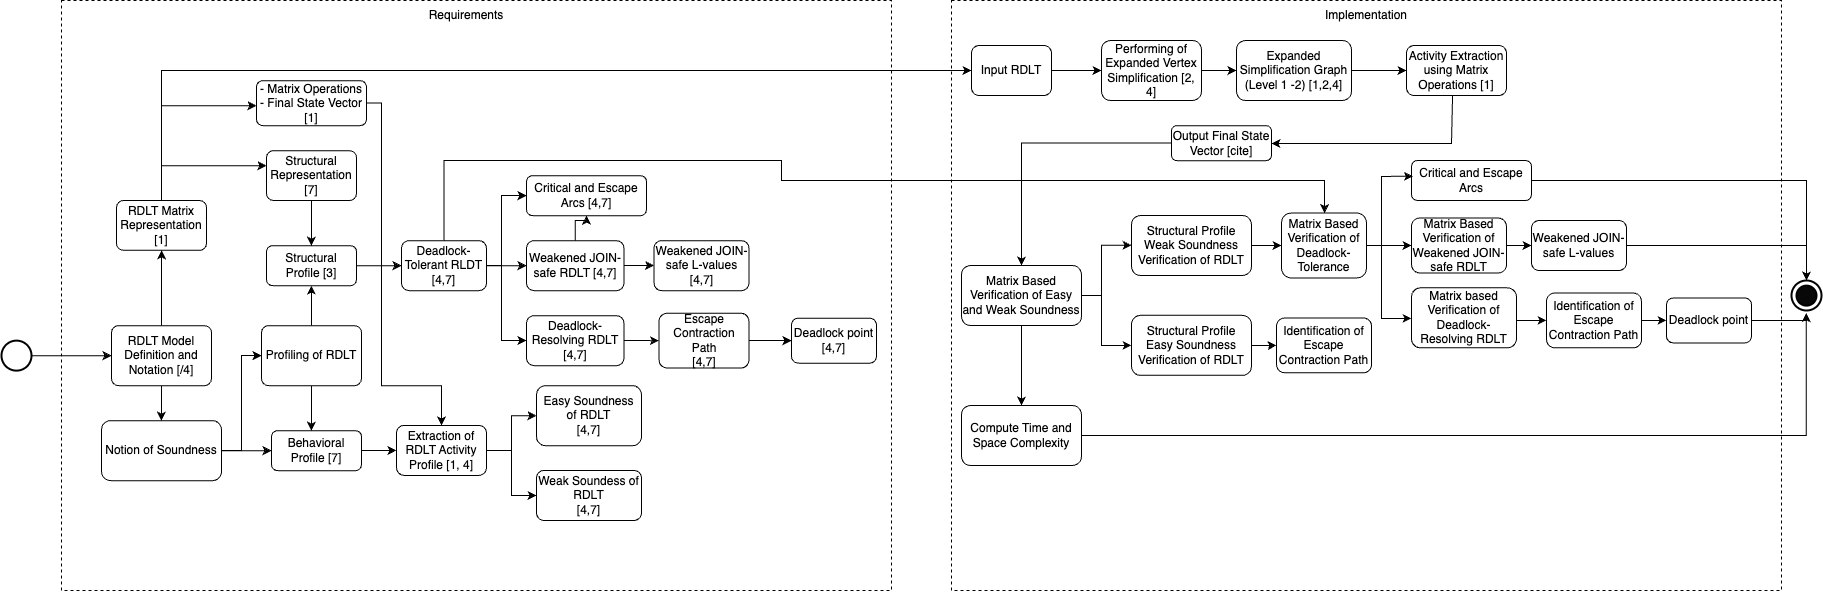
\includegraphics[width=\paperwidth, angle=90]{../figures/Conceptual Framework.png}
    \caption{This framework shows the requirements of the research's framework, with its main components, namely: Matrix Representation, Behavioral and Structural Profile of the RDLT}
\end{figure}